All results are on shapes not used for training or model selection: the test split (301 shapes, 903
volumes per resolution) and the two held-out families (200 shapes each). Table~\ref{tab:main} gives the
overall picture.

\begin{table*}[t]
  \centering\footnotesize
  \caption{Surface-area error (\%) on held-out shapes, all noise levels pooled. MAPE: mean absolute error; bias: mean signed error. The two right-hand blocks are shape families never seen in training (MAPE). Best value per column in bold.}
  \label{tab:main}
  \setlength{\tabcolsep}{3.5pt}
  \begin{tabular}{lrrrrrrrr}
    \toprule
    & \multicolumn{2}{c}{Test MAPE} & \multicolumn{2}{c}{Test bias} & \multicolumn{2}{c}{Superellipsoid} & \multicolumn{2}{c}{Rough blob} \\
    \cmidrule(lr){2-3}\cmidrule(lr){4-5}\cmidrule(lr){6-7}\cmidrule(lr){8-9}
    Method & $32^3$ & $64^3$ & $32^3$ & $64^3$ & $32^3$ & $64^3$ & $32^3$ & $64^3$ \\
    \midrule
    Voxel faces & 56.71 & 65.54 & $+$56.64 & $+$65.54 & 57.45 & 64.81 & 55.30 & 65.65 \\
    MC (binary) & 10.38 & 14.49 & $+$9.56 & $+$14.49 & 10.51 & 14.31 & 8.91 & 13.99 \\
    MC (greyscale) & 4.78 & 3.52 & $-$1.25 & $+$2.41 & 4.10 & 3.38 & 5.27 & 3.57 \\
    MC (smoothed) & 13.78 & 3.04 & $-$13.78 & $-$3.04 & 9.93 & 2.29 & 14.02 & 4.37 \\
    \midrule
    MC + lookup & 2.97 & 0.79 & $-$1.45 & $-$0.46 & 1.87 & 0.43 & 3.22 & 1.09 \\
    Random Forest & 0.72 & \textbf{0.18} & $-$0.18 & \textbf{$+$0.04} & \textbf{0.73} & \textbf{0.39} & \textbf{1.71} & \textbf{0.48} \\
    PointNet & 1.98 & 1.04 & $+$0.33 & $+$0.34 & 1.54 & 0.95 & 3.00 & 1.32 \\
    3D CNN & \textbf{0.68} & 0.26 & \textbf{$-$0.10} & $+$0.10 & 1.05 & 0.45 & 1.96 & 0.55 \\
    \bottomrule
  \end{tabular}
\end{table*}


\subsection{Classical estimators}
Voxel-face counting overestimates the area by 57\% at $32^3$ and 66\% at $64^3$, more than the 50\% of
the theory because noise adds isolated voxels whose faces also count. Binary marching cubes has a
positive bias ($+9.6\%$ at $32^3$, $+14.5\%$ at $64^3$) that grows with resolution instead of shrinking.
The resolution sweep (Fig.~\ref{fig:sweep}) shows why: on clean data the bias rises from $+0.5\%$ at
$24^3$ to $+8.5\%$ at $128^3$, as the theory predicts, and at $\sigma_n=0.15$ from $+16\%$ to $+34\%$,
because more voxels means more noise specks. Greyscale marching cubes is too small for small objects
($-22.9\%$ at $16^3$ on clean data, from curvature) and too large at high noise ($+8.6\%$ at $64^3$).
Because these effects have opposite signs, its error is not smallest on clean data. Smoothing removes
most of the noise error at $64^3$ but costs 13.8\% at $32^3$, where most objects are small.

\begin{figure}[t]
  \centering
  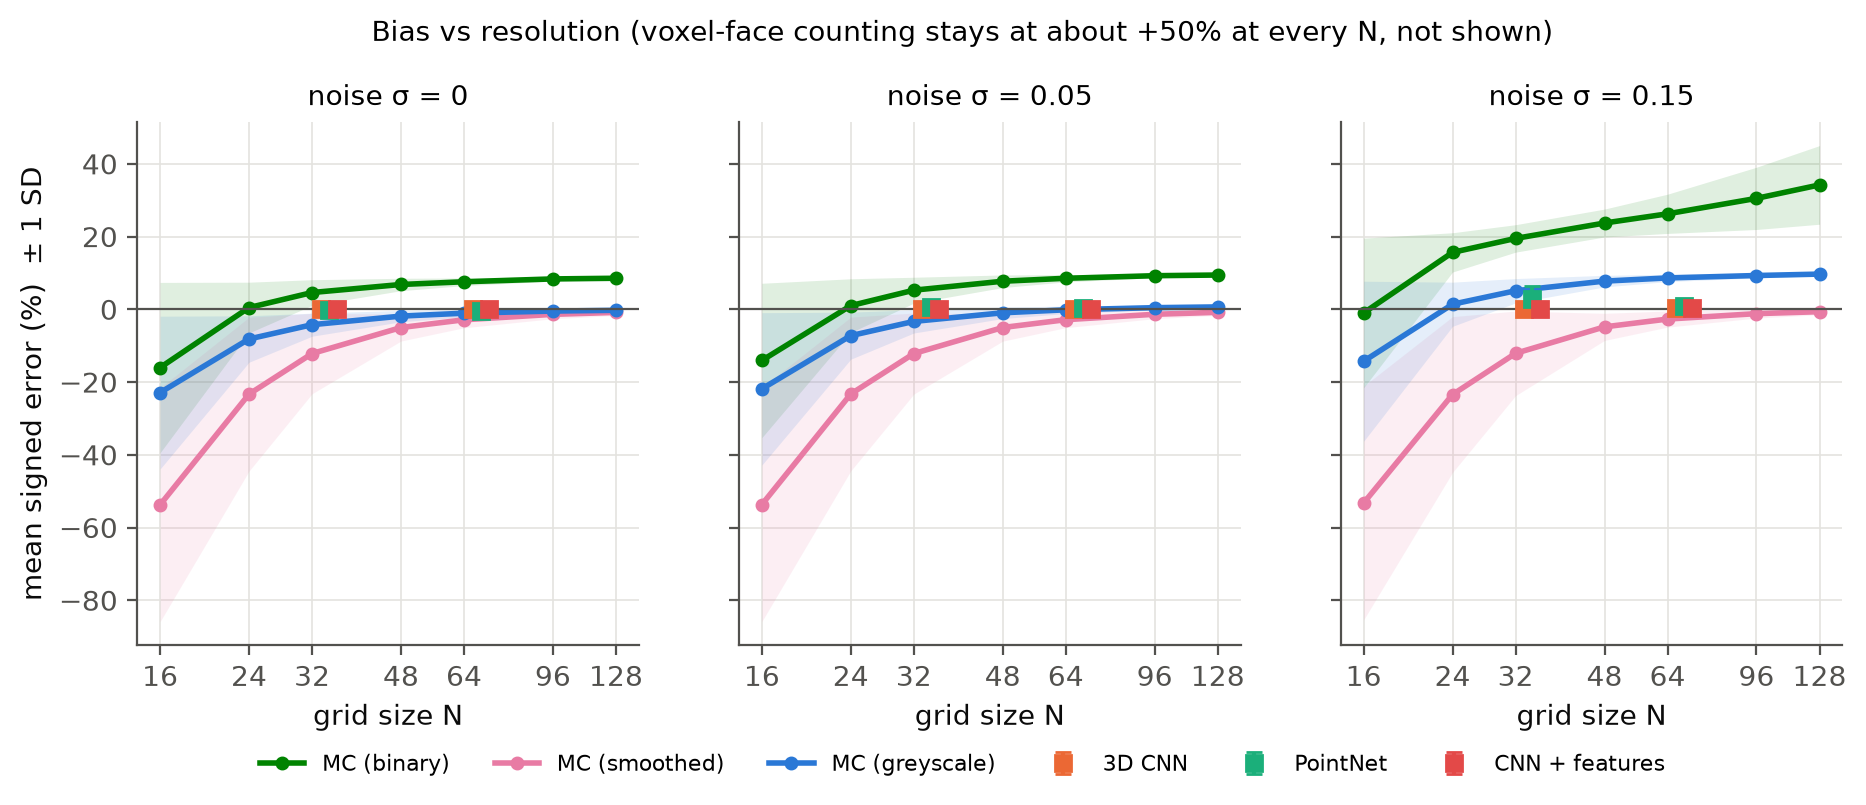
\includegraphics[width=\linewidth]{bias_vs_resolution.png}
  \caption{Mean signed error ($\pm$1 s.d.) of the marching-cubes estimators against grid size for 48
  test shapes. Learned models are shown at the two sizes they were trained on.}
  \label{fig:sweep}
\end{figure}

\subsection{Learned and calibrated corrections}
Every correction improves on raw greyscale marching cubes by a large factor. The lookup table already
reduces the test MAPE from 4.78\% to 2.97\% at $32^3$ and from 3.52\% to 0.79\% at $64^3$, so most of the
error at $64^3$ is a systematic, regime-dependent bias, while at $32^3$ it depends on the individual
object. The 3D CNN reaches 0.68\% and 0.26\%, a seven-fold and a thirteen-fold reduction, with a bias
within $\pm0.1\%$. The Random Forest performs almost identically at $32^3$ (0.72\%) and is the best
model at $64^3$ (0.18\%). Its most important inputs are the Euler number (0.29), the noise estimate (0.26), the smoothed-to-raw marching-cubes area ratio (0.22) and the face-count-to-marching-cubes area ratio (0.08).
The first two
measure exactly the two noise effects of Section~\ref{sec:theory}. PointNet is clearly weaker (1.98\%
and 1.04\%), because sampling points from a mesh that already contains the noise artefacts throws away
the intensity information the volume-based models use.

\subsection{Noise and object size}
The learned models are nearly insensitive to noise (Table~\ref{tab:noise}): at $64^3$ the CNN's MAPE
goes from 0.20\% on clean data to 0.40\% at $\sigma_n=0.15$, while greyscale marching cubes goes from
1.13\% to 8.56\%. Object size matters more than grid size. For objects less than 16 voxels across,
greyscale marching cubes has a MAPE of 6.43\%, the Random Forest 1.41\% and the CNN 1.24\%, the size
class where the CNN has its clearest advantage. Above 48 voxels the Random Forest reaches 0.08\%.

\begin{table}[t]
  \centering\footnotesize
  \caption{Test MAPE (\%) by resolution and noise level. Best per column in bold.}
  \label{tab:noise}
  \setlength{\tabcolsep}{3.5pt}
  \begin{tabular}{lrrrrrr}
    \toprule
    & \multicolumn{3}{c}{$32^3$} & \multicolumn{3}{c}{$64^3$} \\
    \cmidrule(lr){2-4}\cmidrule(lr){5-7}
    Method & $\sigma_n{=}0$ & $0.05$ & $0.15$ & $0$ & $0.05$ & $0.15$ \\
    \midrule
    Voxel faces & 44.10 & 45.64 & 80.38 & 48.31 & 49.91 & 98.40 \\
    MC (binary) & 5.24 & 5.85 & 20.05 & 7.64 & 8.49 & 27.34 \\
    MC (greyscale) & 4.73 & 3.84 & 5.77 & 1.13 & 0.86 & 8.56 \\
    MC (smoothed) & 13.87 & 13.82 & 13.65 & 3.11 & 3.09 & 2.93 \\
    \midrule
    MC + lookup & 3.06 & 3.05 & 2.80 & 0.84 & 0.83 & 0.71 \\
    Random Forest & 0.49 & 0.61 & 1.07 & \textbf{0.09} & \textbf{0.14} & \textbf{0.30} \\
    PointNet & 1.42 & 1.41 & 3.13 & 0.75 & 0.69 & 1.67 \\
    3D CNN & \textbf{0.46} & \textbf{0.55} & \textbf{1.02} & 0.20 & 0.19 & 0.40 \\
    \bottomrule
  \end{tabular}
\end{table}


\subsection{Unseen shape families and a failure case}
Both held-out families stay far below the classical errors (Fig.~\ref{fig:heldout}). On
superellipsoids, whose sharp edges do not occur in training, the CNN reaches 1.05\% and 0.45\% and the
Random Forest 0.73\% and 0.39\%, against 4.10\% and 3.38\% for greyscale marching cubes. Rough blobs are
the hardest case (CNN 1.96\%, Random Forest 1.71\% at $32^3$), with corrections biased low: the models
were trained on smooth shapes and cannot add back area hidden in sub-voxel roughness. At $64^3$ the
error falls to about 0.5\%.

The error distributions are heavy-tailed at $32^3$. The worst case is a test torus whose tube is 1.77
voxels thick: after blurring most of the tube stays below the iso-level, so greyscale marching cubes
recovers only 42 of its 142 voxel$^2$, and every model is off by 47\% to 66\%. A correction of the
marching-cubes area cannot recover a surface that is missing from the mesh.

\begin{figure}[t]
  \centering
  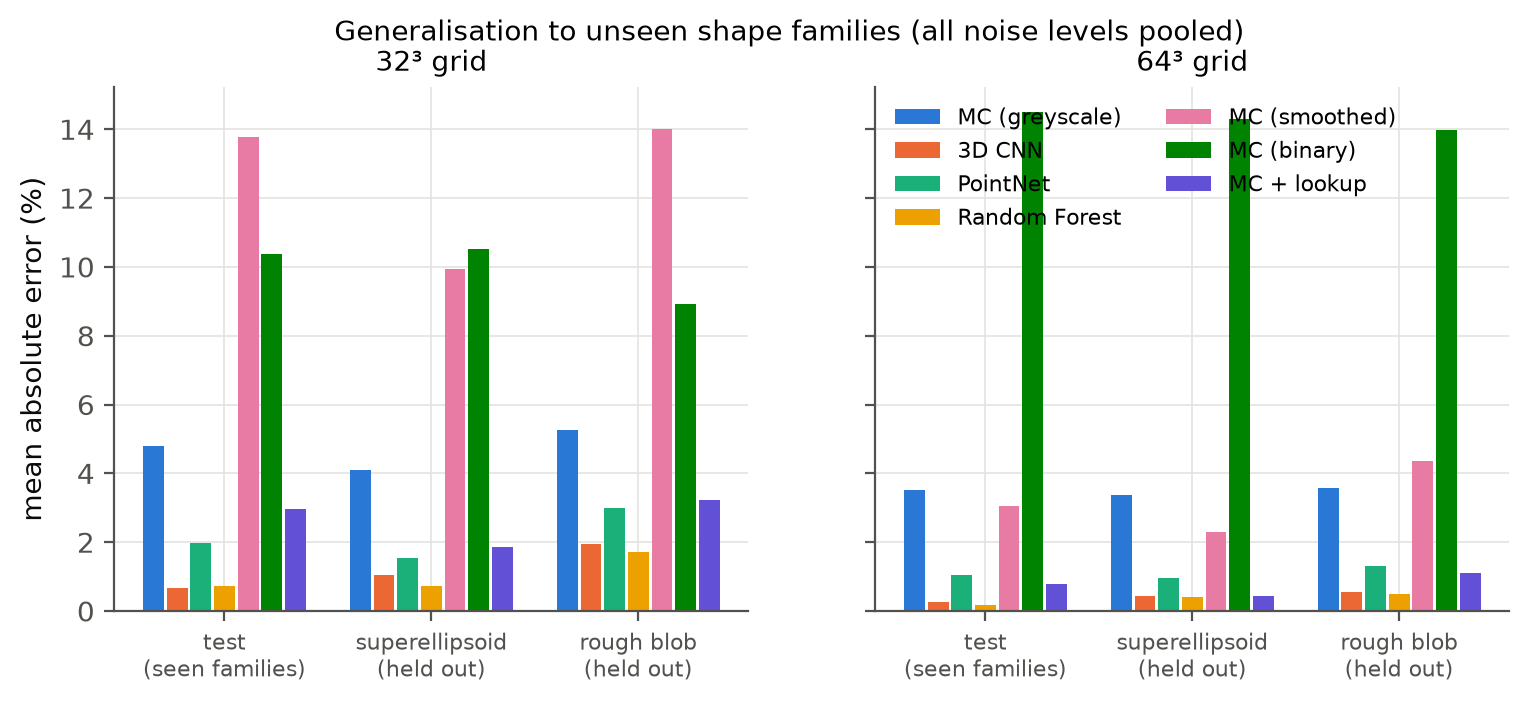
\includegraphics[width=\linewidth]{heldout_families.png}
  \caption{MAPE on the test split and on the two held-out families (all noise levels pooled).}
  \label{fig:heldout}
\end{figure}

\subsection{Which estimator to use}
Table~\ref{tab:regime} summarises when a learned correction is worth the effort. Its benefit is largest
where the classical methods are weakest: small objects, coarse grids and noisy data.

\begin{table}[t]
  \centering\small
  \caption{Recommended estimator by regime, based on the test results.}
  \label{tab:regime}
  \begin{tabular}{p{4.2cm}p{10cm}}
    \toprule
    Regime & Recommendation \\
    \midrule
    Any case & Do not use voxel-face counting or binary marching cubes for absolute area. \\
    Clean data, large objects & Greyscale marching cubes is within about 1\% at $64^3$. \\
    Noisy data ($\sigma_n=0.15$) & A learned correction (CNN or Random Forest) gives 0.3--1.1\%. \\
    Small objects ($<16$ voxels) & Use the 3D CNN (1.24\%, against 6.43\% for marching cubes). \\
    Thinner than about 2 voxels & No method tested here is reliable. \\
    \bottomrule
  \end{tabular}
\end{table}
